\chapter{实例引导的相关滤波器}\label{chap:IGCF}

\section{摘要}
基于传统相关滤波器(CF)的跟踪器通常仅依靠岭回归进行在线学习,而不会感知目标在语义级别的实例信息。这种语义信息的缺乏可能导致跟踪漂移或跟踪器完全失效。为了解决这一问题,我们提出了实例引导的相关滤波器(IGCF),以提高跟踪的鲁棒性。具体来说,一个深层网络(即 InstMask)旨在为目标生成实例掩码,该掩码用于约束相关滤波器的学习。在实例级分割的基础上,我们进一步提出了一种自校正机制来缓解相关滤波跟踪器的漂移问题。在几个具有挑战性的基准测试上进行的广泛实验表明,与最新的跟踪器相比,我们所提出的实例引导的相关滤波跟踪器表现出色,在单个 CPU 内核上的运行速度可达 5 帧每秒。

\section{引言}
目标跟踪是计算机视觉中的基本主题。给定视频起始帧中的初始化目标,跟踪的目的是估计后续帧中目标的状态。尽管在这方面进行了长期的努力,例如 \cite{Leang2018OnlineFO, Wang2019VisualOT, Zhang2018UsingFL},但在低成本平台上仍难以实现可接受的跟踪精度和速度。跟踪过程中的遮挡、照明变化、表观变化和快速运动等现象,使得在自动驾驶,机器人技术和增强现实等现实应用中难以进行跟踪。

在过去的十年中,判别性相关滤波器(DCF)跟踪器 \cite{bolme2010visual, Zhang2018VisualTU} 引起了人们的极大兴趣,该跟踪器通过利用离散傅立叶变换以有效的方式利用了跟踪样本的所有空间偏移。但是,对于大多数 DCF 跟踪器,目标位置由一个矩形框描述。因此,矩形物体区域,特别是用于不规则形状的物体或具有空心中心的物体,将被掺杂大量的背景信息,这可能导致跟踪漂移和故障。此外,DCF跟踪器没有实例级语义信息。信息的缺乏限制了它们的潜力。

基于 DCF 跟踪器的成功,许多研究 \cite{Danelljan2015LearningSR, Lukezic2017DiscriminativeCF} 已证明目标上的空间约束可改善相关滤波器的学习。但是,大多数空间约束都是手工设计的,仍然没有考虑有关目标的语义信息。尽管实例级语义分割 \cite{Pinheiro2015LearningTS, Zhang2019ProgressivelyDN}(旨在为图像中的每个像素分配语义标签)能够提取图像中的实例级语义信息,直接集成现有的实例分割方法以提供空间,相关滤波器学习的约束仍然很难在跟踪精度和速度之间取得平衡。

\iffalse
\begin{figure}
\centering
    \subfloat{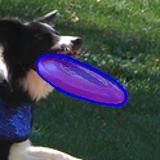
\includegraphics[width=2.4cm]{Img/IGCF/coco/00893.jpg}}          \hspace{-0.6em}        
    \subfloat{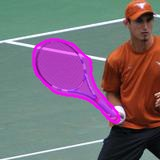
\includegraphics[width=2.4cm]{Img/IGCF/coco/01107.jpg}}          \hspace{-0.6em}        
    \subfloat{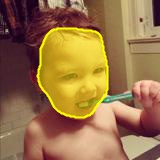
\includegraphics[width=2.4cm]{Img/IGCF/coco/01108.jpg}}          \hspace{-0.6em}        
    \subfloat{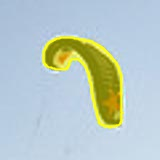
\includegraphics[width=2.4cm]{Img/IGCF/coco/01564.jpg}}          \hspace{-0.6em}        
    \subfloat{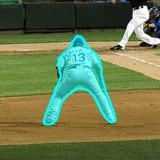
\includegraphics[width=2.4cm]{Img/IGCF/coco/01664.jpg}}\\[0.2ex]
    \subfloat{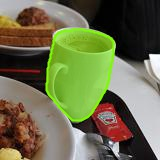
\includegraphics[width=2.4cm]{Img/IGCF/coco/01939.jpg}}                     \hspace{-0.6em}
    \subfloat{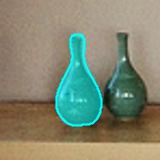
\includegraphics[width=2.4cm]{Img/IGCF/coco/02078.jpg}}                     \hspace{-0.6em}
    \subfloat{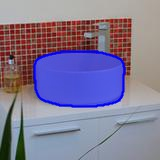
\includegraphics[width=2.4cm]{Img/IGCF/coco/02285.jpg}}                     \hspace{-0.6em}
    \subfloat{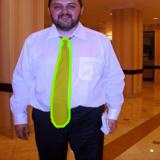
\includegraphics[width=2.4cm]{Img/IGCF/coco/02497.jpg}}                     \hspace{-0.6em}
    \subfloat{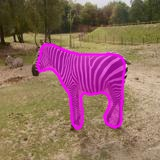
\includegraphics[width=2.4cm]{Img/IGCF/coco/02589.jpg}}\\[0.2ex]
    \subfloat{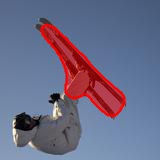
\includegraphics[width=2.4cm]{Img/IGCF/coco/02700.jpg}}                   \hspace{-0.6em}
    \subfloat{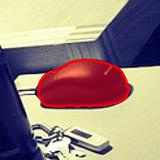
\includegraphics[width=2.4cm]{Img/IGCF/coco/03000.jpg}}                   \hspace{-0.6em}
    \subfloat{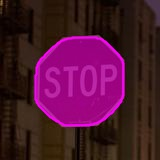
\includegraphics[width=2.4cm]{Img/IGCF/coco/03327.jpg}}                   \hspace{-0.6em}
    \subfloat{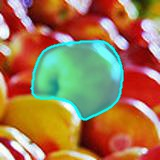
\includegraphics[width=2.4cm]{Img/IGCF/coco/03482.jpg}}                   \hspace{-0.6em}
    \subfloat{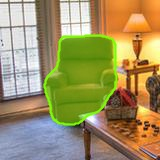
\includegraphics[width=2.4cm]{Img/IGCF/coco/03733.jpg}}
    \caption{InstMask 在 COCO2017 \cite{COCO} 验证集上的分割结果。}
    \label{fig:InstMask}
\end{figure}
\fi

\begin{figure}
\centering
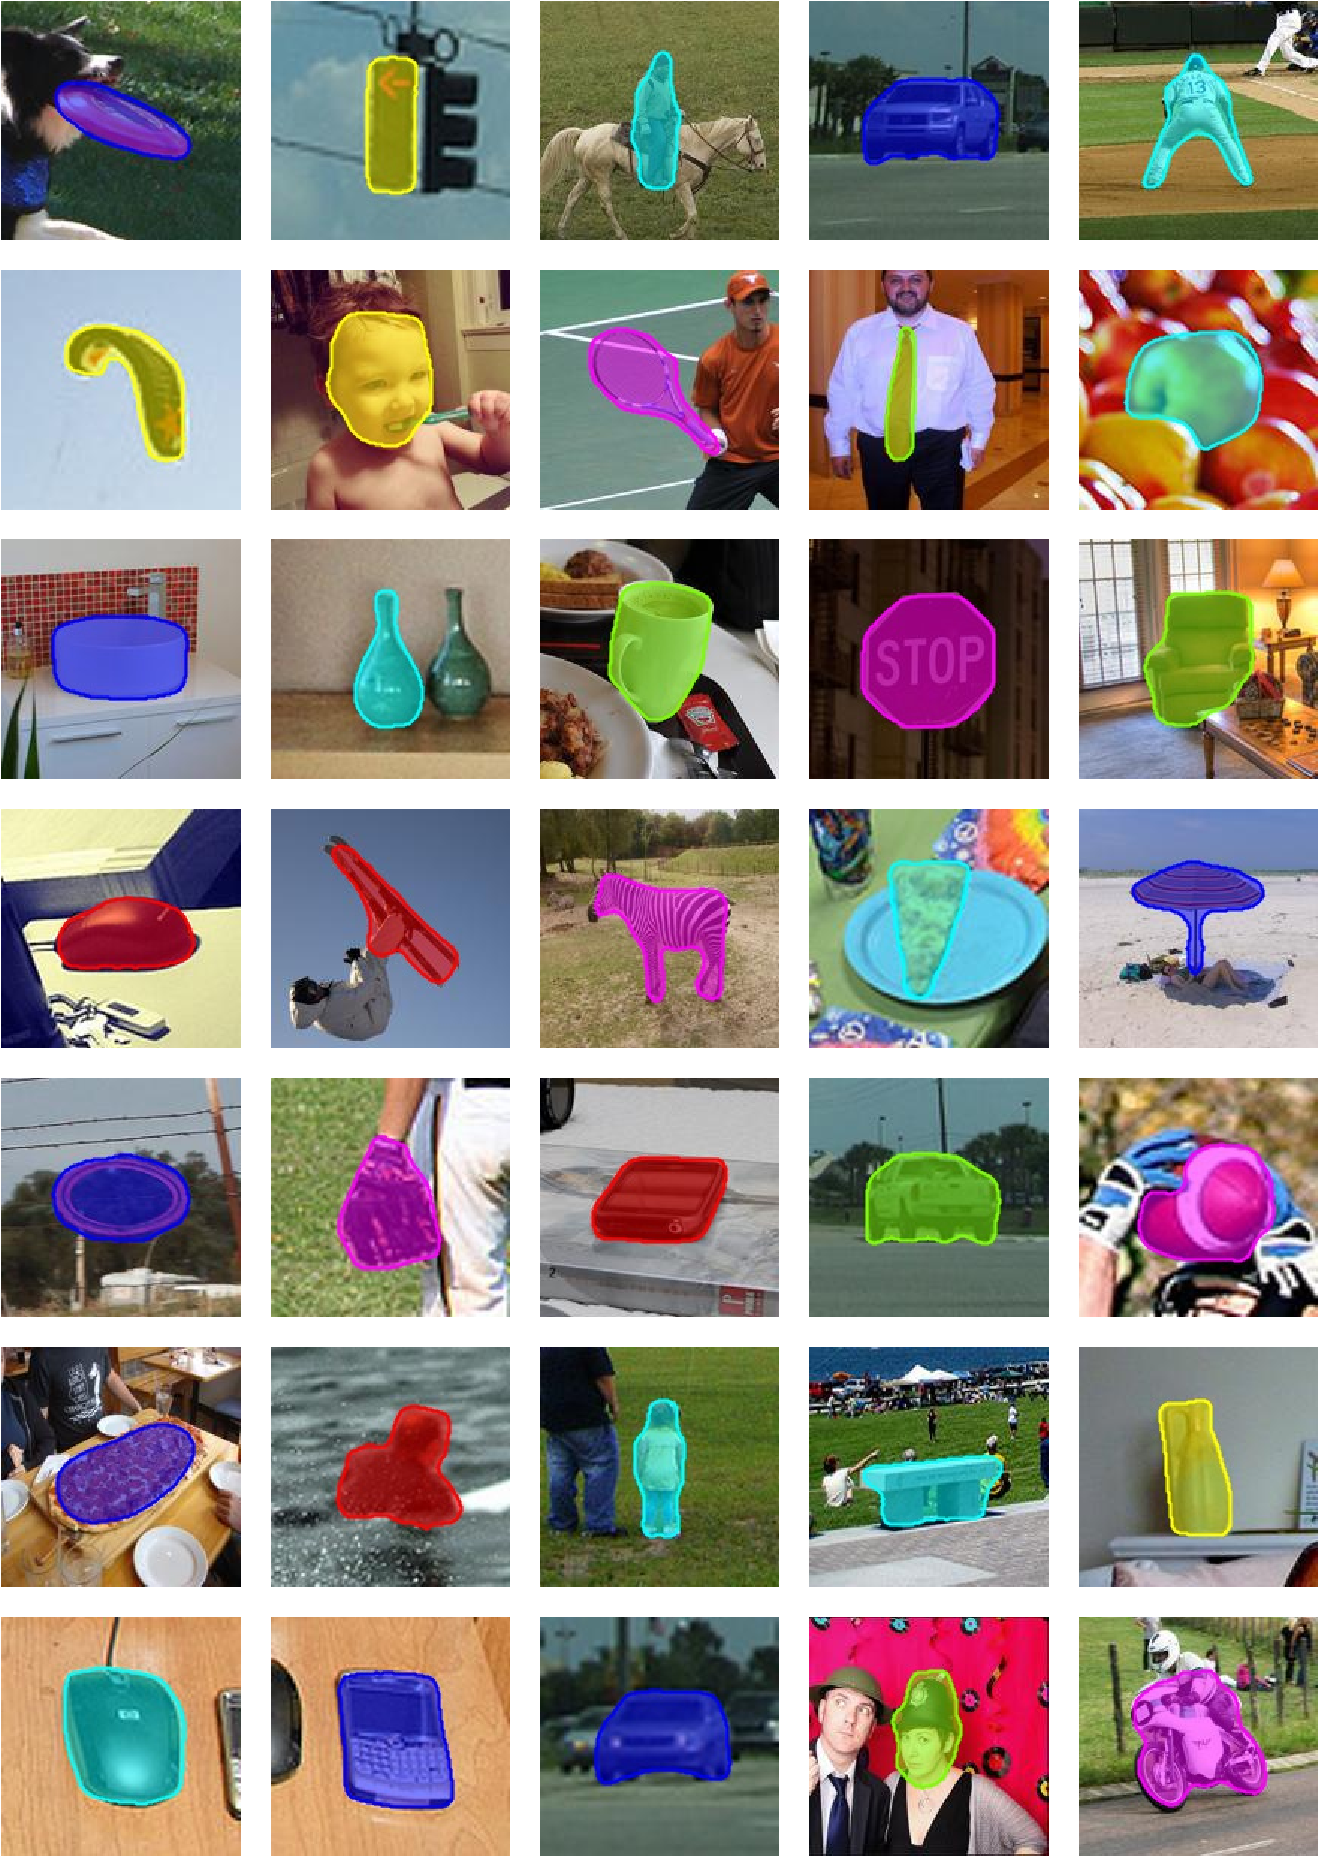
\includegraphics[width=1.0\textwidth]{Img/IGCF/coco.pdf}
\caption{InstMask 在 COCO2017 \cite{COCO} 验证集上的分割结果。}
\end{figure}

在这项工作中,我们提出了实例引导的相关滤波器(IGCF)来解决上述限制。具体而言,我们设计了一个深层卷积神经网络(即InstMask),旨在准确生成目标实例级别的语义分割掩码。我们利用COCO2017 \cite{COCO} 对 InstMask 进行了离线的端到端训练(参见图 \ref{fig:InstMask})。实例级别的语义分割模板可以抑制背景噪声的干扰,从而显式约束相关滤波器的学习过程。
与常见的目标分割任务不同,我们设计了一种新的网络结构和训练方法,使得 InstMask 能够识别位于搜索图像中心附近的任意类别的显著目标。InstMask 可以识别任意类别的目标,而不仅限于识别训练集中出现的类别中的目标。此外,我们的网络由一个 $1 \times 1$ 卷积层构成,可以使全局感受野从目标附近获取上下文信息,这增加了分割的准确性。所提出的轻量级的分割网络可在单个 CPU 核心平台上以 5 FPS 的速度运行时,可以在跟踪精度和速度之间取得平衡。

此外,我们注意到,为满足跟踪自适应性要求而在线更新的相关滤波器与满足鲁棒性要求的离线 InstMask 模块是独立且互补的。因此,两个组件的输出可以集成在一起,以进一步提高跟踪性能。具体而言,基于实例级别的分割,我们进一步提出了一种自校正机制来缓解相关滤波跟踪器的漂移问题。分割掩码的几何中心用于校正相关滤波器的预测偏差。配备了 InstMask 模块,提出的 IGCF 不仅可以精确地跟踪目标,还可以用于视频目标分割,这证明了我们算法的广泛应用。所提出的的跟踪框架 IGCF 的体系结构如图 \ref{fig:IGCF} 所示。

\begin{figure*}
    \centering
    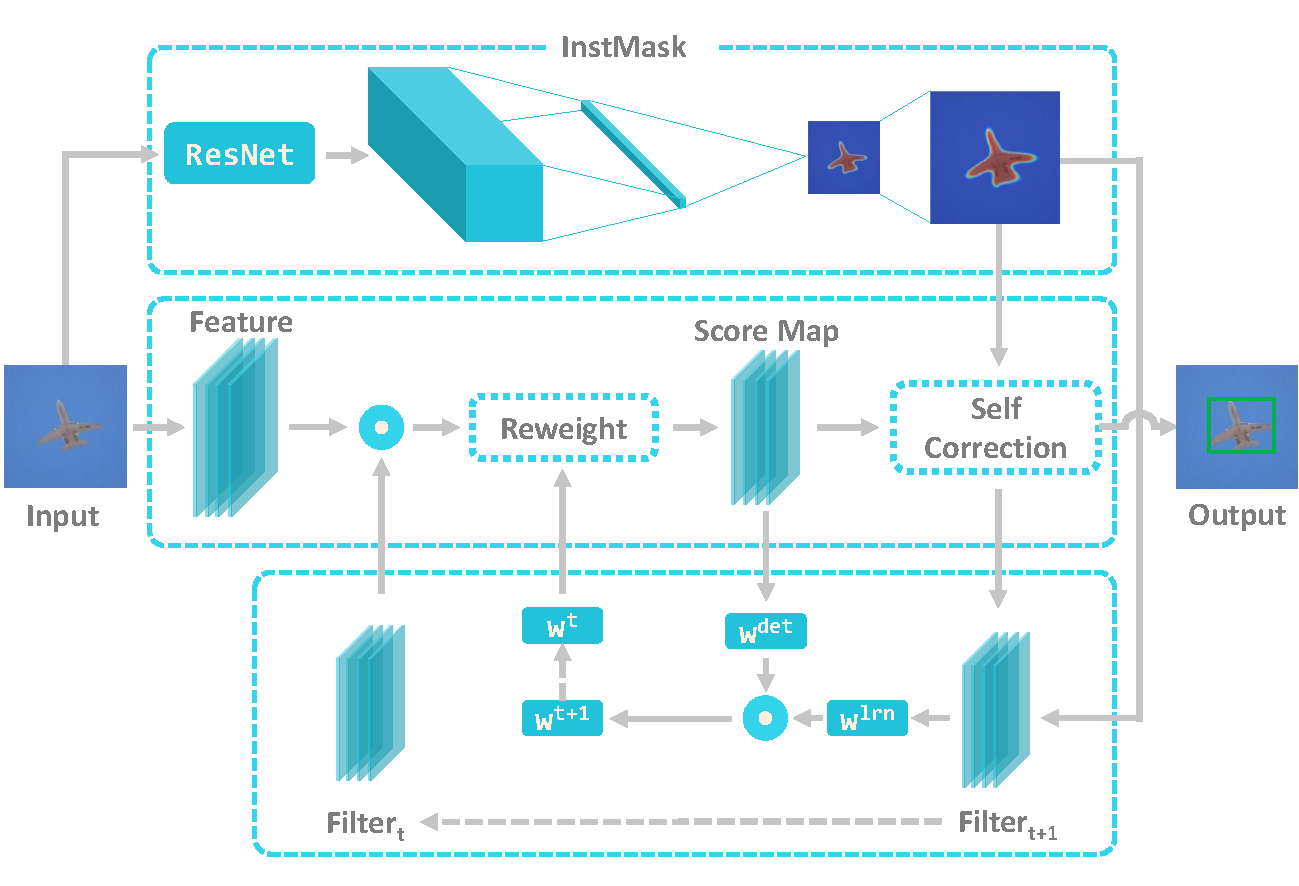
\includegraphics[width=1.0\textwidth]{Img/IGCF/instmask1.pdf}
    \caption{跟踪框架 IGCF 的结构。}
    \label{fig:IGCF}
\end{figure*}

我们在三个跟踪数据库上进行了全面的实验:VOT2015 \cite{Kristan2015TheVO}、VOT2016 \cite{Kristan2016TheVO} 和 GOT-10k \cite{GOT-10k}。我们的 IGCF 跟踪器在跟踪精度方面取得了良好的平衡,同时与最新的跟踪器相比表现出色。最后,我们对视频目标分割数据集 DAVIS2016 \cite{Perazzi2016} 进行了定性实验,以展示我们算法强大的视频语义分割和跟踪功能。

\section{相关工作}
几十年来,目标跟踪一直是热门话题。目标跟踪的目的是在给定目标在第一帧中的位置的情况下,确定目标在视频帧中的位置。

\subsection{基于相关滤波器的跟踪器}
许多基于DCF的跟踪器旨在考虑部分遮挡,照明变化,背景杂波,运动模糊,视点变化等问题。

\cite{bolme2010visual} 等提出基于平方误差最小输出和(MOSSE)滤波器的跟踪器。该跟踪器以每秒 669 帧的速度运行,可以抵抗光照,比例,姿势和非刚性变形的变化。
CSK 跟踪器 \cite{Henriques2012ExploitingTC} 通过采用图像子窗口的循环结构并使用快速傅里叶变换(FFT)快速合并来自所有子窗口的信息,对 MOSSE 跟踪器进行了改进。此外, \cite{Henriques2012ExploitingTC} 表明,使用核技巧可以像在原始图像空间中一样高效地完成非线性空间中的分类。
\cite{Danelljan2014AdaptiveCA} 通过学习有关多维颜色属性的多通道滤镜来改进 CSK 跟踪器。为了避免由于颜色属性的高维而导致的计算开销,\cite{Danelljan2014AdaptiveCA} 提出了一种自适应维降技术,可以将原始的 11 维减少到只有 2 维。
后来,\cite{henriques2014high-speed} 为成千上万个已翻译补丁的数据集提出了一种分析模型。使用离散傅立叶变换将模型对角线化。此操作可以将存储和计算量减少几个数量级。

最近,许多研究 \cite{Danelljan2015LearningSR, Lukezic2017DiscriminativeCF} 已将空间约束引入到相关滤波器的学习中。在 \cite{Danelljan2015LearningSR} 中提出了一种称为“空间正则化差异相关滤波器(SRDCF)”的跟踪器。SRDCF在学习中引入了空间正则化组件,以根据相关滤波器系数的空间位置对它们进行惩罚。
此外,\cite{Lukezic2017DiscriminativeCF} 提出的 CSR-DCF 滤波器将通道和空间可靠性组件引入了相关滤波跟踪器,并为它们在滤波器更新和跟踪过程中的有效无缝集成提供了学习算法。空间可靠性组件将滤波器支撑调整到目标的合适部分。通道可靠性组件根据特征的位置生成特征加权系数。CSR-DCF 跟踪器具有较大的搜索区域,可以有效跟踪非矩形目标。空间可靠性组件与 Staple(模板和 Pixelwise 学习器的总和) \cite{Bertinetto2016StapleC} 跟踪器中使用的颜色分布具有一些相似之处。该跟踪器结合了补充提示,以提高鲁棒性。它解决了关于基于相关滤波器的模板模型和逐像素颜色分布模型的两个独立的岭回归问题。
为了处理目标的尺度变化, \cite{Li2014ASA} 中提出的方法以不同的尺度对目标进行采样,并将采样调整为固定大小,以与每个帧上的学习模型相匹配。此方法还采用了多特征集成方案,该方案使用原始像素,渐变直方图 \cite{Forsyth2014ObjectDW} 和颜色命名 \cite{Weijer2009LearningCN} 来进一步增强跟踪器。这些基于DCF的跟踪器的主要缺点是缺乏对目标的高级语义信息的感知。

\subsection{基于卷积神经网络的跟踪器}
在过去的几年中,深度学习 \cite{Goodfellow2015DeepL} 在许多研究领域都取得了显著成功,尤其是在计算机视觉 \cite{Matiz2019InductiveCP, Zhu2019RotatedCR, Xiao2019DenseSE},语音识别 \cite{Kim2016JointCB, Liu2019AttentionGD}和自然语言处理 \cite{Vinyals2014GrammarAA, Yousfi2017ContributionOR} 等领域。一些跟踪器已经证明了深度学习的性能优势。

大多数基于 DCF 的跟踪器仅限于单分辨率特征图,从而极大地限制了其潜力。为了解决此问题,CCOT跟踪器 \cite{CCOT} 学习连续卷积滤波器以融合以不同分辨率获得的特征图。这将为目标生成连续域置信度图。除了多分辨率融合之外,连续域学习公式还可以实现精确的亚像素定位。
ECO 跟踪器 \cite{Danelljan2017ECOEC} 在核心 DCF 公式中包括分解卷积算子,训练样本分布的紧凑生成模型和保守模型更新策略。由于使用了 CNN 特征,这减轻了计算开销。相反,CF2 跟踪器 \cite{Ma2015HierarchicalCF} 自适应地学习每个卷积层上的相关滤波器,以对目标外观进行编码,并使用每一层的相关响应来推断目标位置。

\cite{GOTURN} 提出了一种离线训练的神经网络来进行跟踪目标。他们使用简单的前馈网络,而无需在线训练。该网络了解对象运动与外观之间的一般关系,并可用于跟踪未出现在训练集中的新颖对象。
最近,一系列跟踪器,例如SiamFC \cite{SiamFC},SiamRPN \cite{SiamRPN},DasiamRPN \cite{zhu2018distractor} 和SiamMask \cite{Wang2018SiamMask},使用孪生网络来学习搜索图像和模板图像之间的相似性。它们在跟踪速度和准确性之间取得了良好的平衡。SiamMask 是在一个端到端学习框架中同时执行跟踪和分割的首次尝试。
尽管在准确性和鲁棒性方面都具有吸引人的性能,但是上述大多数跟踪器都具有很高的特征提取计算开销,因此不适合于低成本平台。例如,SiamMask 算法在Intel E5-2620 CPU平台上仅以 1 FPS 运行。

也有一些工作致力于使用自校正机制来减轻跟踪漂移,从而提高跟踪的鲁棒性。例如,在 \cite{fan2018parallel} 中,跟踪框架由两个组件(跟踪器和验证器)组成,它们在两个单独的线程上并行工作。跟踪器提供实时跟踪推断,并有望在大多数情况下表现良好。相反,验证者检查跟踪结果并在需要时更正跟踪器。

\section{方法}

\subsection{跟踪范式}
DCF 跟踪器 \cite{Danelljan2014AccurateSE, henriques2014high-speed, Li2014ASA} 已得到广泛研究和使用。具体来说,考虑目标的表观特征:$f=\{f_d\}_{d=1:N_c}$ ,其中 $N_c$ 是目标特征的通道号。类似于 DCF 跟踪器的目标是训练滤波器 $h=\{h_d\}_{d=1:N_c}$,以使特征和滤波器之间的相关性响应 $\tilde{g}$ 适合所需输出 $g$ ,通常是一个以目标位置为中心的二维高斯函数: 
\begin{equation} \label{eq:dcf}
\tilde{g}=\sum_{d=1}^{N_c}f_d \star h_d \cdot w_d,
\end{equation}
其中 $\star$ 表示循环相关运算符,通道权重 $w = \{w_d\}_{d=1:N_c}$ 是基于每个特征通道 \cite{Lukezic2017DiscriminativeCF}.
的判别力的缩放因子。
响应图的峰值位置是目标在当前帧中的估计位置。
最佳相关滤波器 $h$ 通过最小化来估算:
\begin{equation}
\varepsilon(h) = \sum_{d=1}^{N_c}||f_d \star h_d - g||^2+\lambda||h_d||^2.
\end{equation}

最近,许多研究 \cite{Danelljan2015LearningSR, Lukezic2017DiscriminativeCF} 已经证明,强加于目标的空间约束通过减少背景干扰来改善相关滤波器学习。如 \cite{Lukezic2017DiscriminativeCF}中所述,图像补丁的分割掩码是一个元素为 1 或 0 的空间图,用于指示像素是属于目标还是属于背景。在滤波器的训练过程中,滤波器 $h$ 受掩码 $m$ 约束:$h \equiv m \odot h$,其中 $\odot$ 表示 Hadamard(逐元素)乘积。该约束使滤波器支持适合目标的适合跟踪的部分。这使得可以使用较大的训练区域来捕获更多上下文信息,并克服了矩形框的局限性。

\subsection{InstMask}
\label{sec:InstMask}
在本文中,我们使用被跟踪的目标的分割掩码来约束相关滤波器的学习。出于效率和性能方面的考虑,理想的分割方法应具有三个关键特征:

\begin{itemize}
\item 与跟踪过程的无缝集成;
\item 足够简单以适应跟踪的速度要求;
\item 设计的分割算法应尽可能准确地预测目标的轮廓。
\end{itemize}

以前大多数用于生成空间约束的方法都依赖于手工设计的规则或低级图像特征(例如颜色直方图)。
在本文中,我们介绍了 InstMask 网络,该网络为目标生成准确的实例掩码。我们使用数据驱动的方法对 InstMask 进行离线地端到端训练,以从分割训练集中学习语义信息,例如 COCO2017 \cite{COCO}。实例级别的语义分割掩码可以通过抑制背景杂波来限制相关滤波器的学习。在实例级分割的基础上,我们进一步提出了一种自校正机制来减轻相关滤波跟踪器的漂移问题。与传统的相关滤波跟踪方法相比,此方法可显着提高目标跟踪精度。
与以前的生成分割掩码的方法不同,我们不依赖于边缘,超像素或其他形式的低级分割。相反,我们模型的核心是卷积神经网络。通过利用在 ImageNet \cite{ImageNet} 上训练的强大卷积特征表示并适应 COCO 中可用的大量分割训练数据,我们能够为目标生成语义分割掩码,以限制相关跟踪器的学习。
值得注意的是,将现有的实例分割方法进行集成以为相关滤波器学习提供空间约束是次优的。通用跟踪算法通常具有复杂的网络结构,因此很难在跟踪精度和速度之间取得平衡。相比之下,本文提出的分割网络是专为跟踪而设计的,重量很轻,在 CPU 上以 5 FPS 运行。

当在第 $i$ 帧中跟踪时,需要获得帧 $i$ 中目标的分割掩码以约束相关滤波器的学习。
假定 $i$ 帧中的目标位置在 $i-1$ 帧中的目标位置附近,因此 InstMask 的输入始终是前一帧以对象位置为中心的小图像区域。
该设计具有以下优点:

\begin{itemize}
\item 由于输入数据的强一致性,网络可以使用较少的参数获得准确的分割结果。
\item 由于网络参数较少且图像补丁较小,因此推理时间短。
\item 在目标的先前位置附近进行搜索可以避免位于后台的干扰因素的不利影响。在训练期间,训练集中的每个样本 $k$ 包含(1)RGB输入色块 $x_k$,其中包含接近输入色块中心的目标,(2)对应的二进制掩码 $m_{k}$ 输入补丁。
\end{itemize}

接下来,我们描述体系结构和训练过程。

\textbf{体系结构} 表 \ref{tab:InstMask} 和图 \ref{fig:net} 中显示了网络体系结构。InstMask 的主干是基于 ResNet50 \cite{He2016DeepRL} 构建的,它由一个主干块和3个残差块组成。
InstMask 的输入是一个 160$\times$160$\times$3 图像补丁。它被发送到主干块,生成尺寸为 40$\times$40$\times$64 的特征图。然后将特征图顺序发送到3个残差块,分别生成大小为 40$\times$40$\times$256, 20$\times$20$\times$512, 10$\times$10$\times$1024 的特征图。随后,将获得的特征图发送到三个卷积层以生成长度为 3136 的向量,该向量使全局接收场能够感知有关目标的所有上下文信息。最后,将此向量尺寸调整为 56$\times$56,以获得最终的分割掩码。由于它是一个轻量级的网络,因此我们建议的跟踪方法可以在具有 Intel E5-2620 CPU 内核的平台上以 5 FPS 运行,以最佳地平衡跟踪准确性和速度,从而可以将跟踪器部署在包括自动控制在内的实际应用中驾驶,机器人技术和增强现实。

\begin{algorithm}[t]
  \caption{IGCF 跟踪算法} 
  \begin{algorithmic}
    \Require 图像 $I_t$,目标在上一帧中的位置 $p_{t-1}$、尺度 $s_{t-1}$、滤波器 $h_{t-1}$,通道可靠性 $w_{t-1}$。
    \Ensure 位置 $p_t$,尺度 $s_t$ 和更新后的模型。
  \Statex
  \State \textbf{定位:}
  \begin{enumerate}[leftmargin=0pt,itemindent=1.5em]
    \item $p_t$:$h_{t-1}$ 和从位置 $p_{t-1}$ 提取的图像块的特征 $f_{t}$ 进行相关后的最大响应的位置,由信道可靠性得分加权 $w_{t-1}$(等式 \ref{eq:dcf})。
    \item 估计分割掩码 $m$(第 \ref{sec:InstMask} 节)。
    \item 使用 $m$ 校正 $p_t$ (第 \ref{sec:cog} 节)。
    \item 使用位置 $p_t$ 估计新的尺度 $s_ t$ (参考 \cite{Danelljan2014AccurateSE})。
    \item 使用等式 \ref{eq:det},根据逐通道响应,估计检测可靠性 $\tilde{w}^{(det)}$。
  \end{enumerate}
  \State \textbf{更新:}
  \begin{enumerate}[leftmargin=0pt,itemindent=1.5em]
    \item 使用等式 \ref{eq:h1}至等式 \ref{eq:h3},根据 $m$ 估计新滤波器 $\tilde{h}$。
    \item 使用等式 \ref{eq:lrn},根据 $h$ 估计学习通道可靠性 $\tilde{w}^{(lrn)}$。
    \item 使用等式 \ref{eq:c} 计算通道可靠性 $\tilde{w}$。
    \item 使用等式 \ref{eq:update1} 和等式 \ref{eq:update2} 更新滤波器 $h_t$ 和通道可靠性 $w_t$。
  \end{enumerate}
\end{algorithmic}
\end{algorithm}

\textbf{训练} 在训练期间,将空间分辨率为 56$\times$56 的掩码上采样至原始图像大小 160$\times$160。令 $l$ 表示大小为 $w \times h$ 的逐个像素的真实掩码。损失计算如下:
\begin{equation}
L = \frac{1}{wh} \sum_{xy}{log(1+e^{-l_{x,y}P_{x,y}})},
\end{equation}
其中 $l_{x,y} \in \{ \pm 1 \}$ 是与对象掩码的像素 $(x,y)$ 对应的标签,而 $P_{x,y}$ 是 InstMask 的预测在位置 $(x,y)$。

COCO2017 \cite{COCO} 实例分割数据集用于训练 InstMask。
与许多只能预测训练集中出现的类别的分割网络相反,提出的 InstMask 在训练过程中会忽略类别信息,并作为与类无关的分割网络工作。实际上,InstMask 在搜索区域中检测到显著目标。尽管 InstMask 仅使用 80 个类别的 COCO 数据集 \cite{COCO} 进行训练,但是网络能够将目标分割为训练集中未出现的类别,如图 \ref{fig:IGSC} 所示。
我们使用随机梯度下降训练模型,批次大小为 32,动量为 0.9,权重衰减为 0.00005。总共进行 50 轮迭代训练。学习率在对数空间内从 $10^{-2}$ 减小至 $10^{-4}$。在训练期间,输入图像大小设置为 160$\times$160,目标位于图像的中心,大小为 112$\times$112。为了增强网络的通用性,我们执行数据增强。具体来说,我们考虑平移($\pm$16 像素),缩放变形( $2^{\pm 1/4}$)以及水平翻转。

InstMask 离线训练。在跟踪过程中,InstMask 仅执行前向传播过程,而不会进行梯度的后向传播。这不仅可以防止漂移,还可以满足实时跟踪要求。

尽管我们的模型与 CSRDCF \cite{Lukezic2017DiscriminativeCF}具有高度的相似性,但实现原理却大不相同。
在CSRDCF \cite{Lukezic2017DiscriminativeCF}中,使用目标和背景的颜色直方图生成分割掩码。这种启发式方法具有几个缺点:

\begin{itemize}
\item 由于仅使用低级像素信息,因此难以准确地分割目标。
\item 为了适应目标的明显变化,在跟踪过程中会不断更新直方图模型,这很容易导致跟踪器漂移。
\end{itemize}

相反,InstMask 不会在线更新参数。这提高了计算效率,同时避免了不希望的漂移。此外,由于使用语义级别而不是像素级别的信息进行分割,因此跟踪结果更加准确。

%\setlength\extrarowheight{1pt}
\begin{table}
\centering
\caption{InstMask 的网络结构设计。}
\begin{tabular}{|c|c|c|}
\hline
Layers & Output Size & Support \\\hline
Data & $160 \times 160 \times 3$ &  -\\\hline
\multirow{2}*{Stem Block} & $80 \times 80 \times 64$ &  $ 7 \times 7 \text{ conv} $\\\cline{2-3}
~ & $40 \times 40 \times 64$ &  $ 2 \times 2 \text{ maxpool} $\\\hline
Res Block (1) & $40 \times 40 \times 256$ &  $ \left [ \begin{array}{l} 1 \times 1 \text{ conv} \\ 3 \times 3 \text{ conv} \\ 1 \times 1 \text{ conv} \end{array} \right ] \times 3 $\\\hline
Res Block (2) & $20 \times 20 \times 512$ &  $ \left [ \begin{array}{l} 1 \times 1 \text{ conv} \\ 3 \times 3 \text{ conv} \\ 1 \times 1 \text{ conv} \end{array} \right ] \times 4 $\\\hline
Res Block (3) & $10 \times 10 \times 1024$ &  $ \left [ \begin{array}{l} 1 \times 1 \text{ conv} \\ 3 \times 3 \text{ conv} \\ 1 \times 1 \text{ conv} \end{array} \right ] \times 6 $\\\hline
\multirow{5}*{Decoder} & $10 \times 10 \times 128$ &  $ 1 \times 1 \text{ conv} $\\\cline{2-3}
~ & $1 \times 1 \times 512$ &  $ 10 \times 10 \text{ conv} $\\\cline{2-3}
~ & $1 \times 1 \times 3136$ &  $ 1 \times 1 \text{ conv} $\\\cline{2-3}
~ & $56 \times 56$ & reshape \\\cline{2-3}
~ & $160 \times 160$ & upscale \\\hline
\end{tabular}
\label{tab:InstMask}
\end{table}

\begin{figure*}[t]
    \centering
    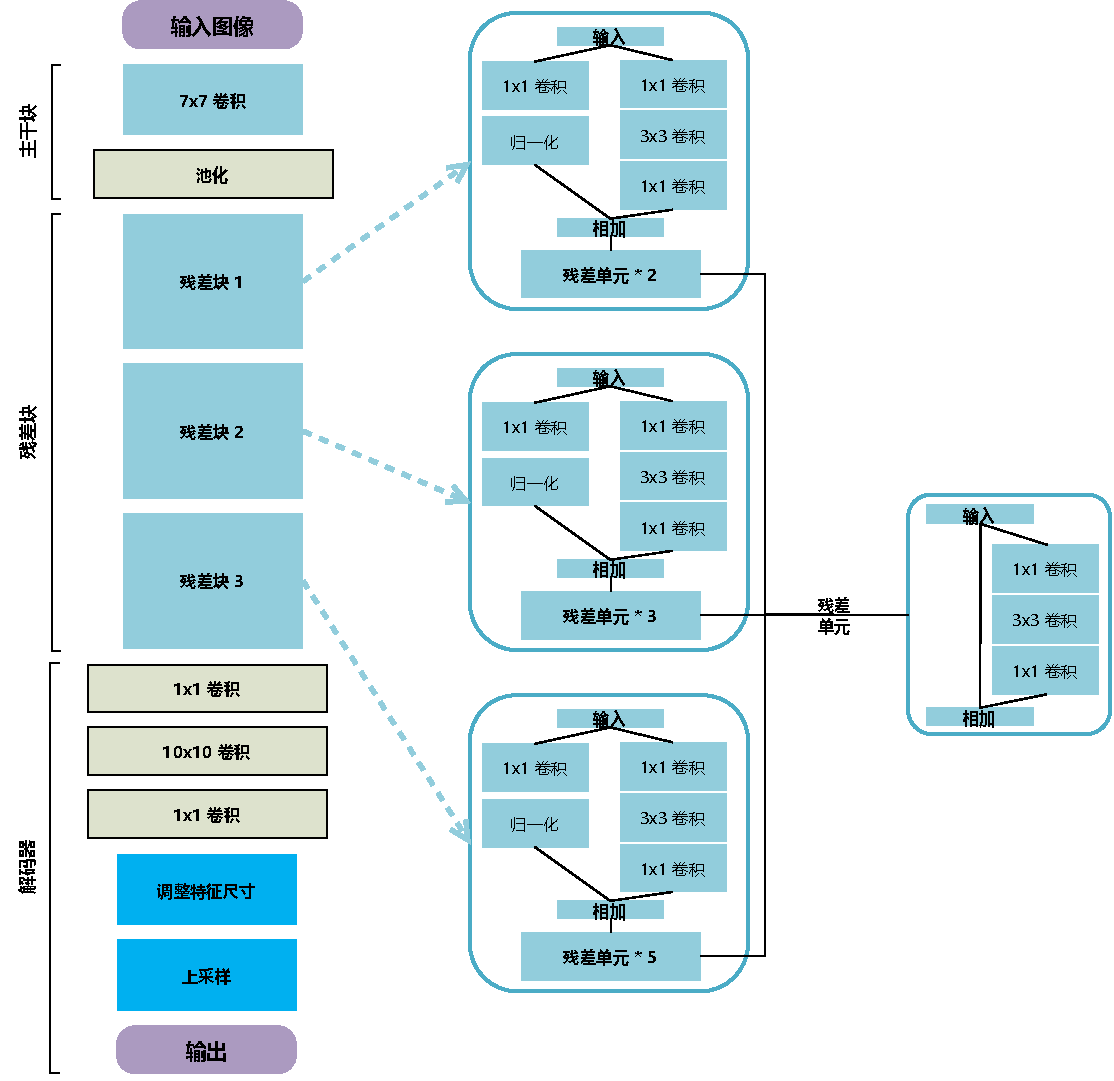
\includegraphics[width=1.0\textwidth]{Img/IGCF/net.pdf}
    \caption{InstMask 的网络结构。}
    \label{fig:net}
\end{figure*}

\subsection{实例引导的自纠正组件} \label{sec:cog}

\begin{figure*}[t]
    \centering
    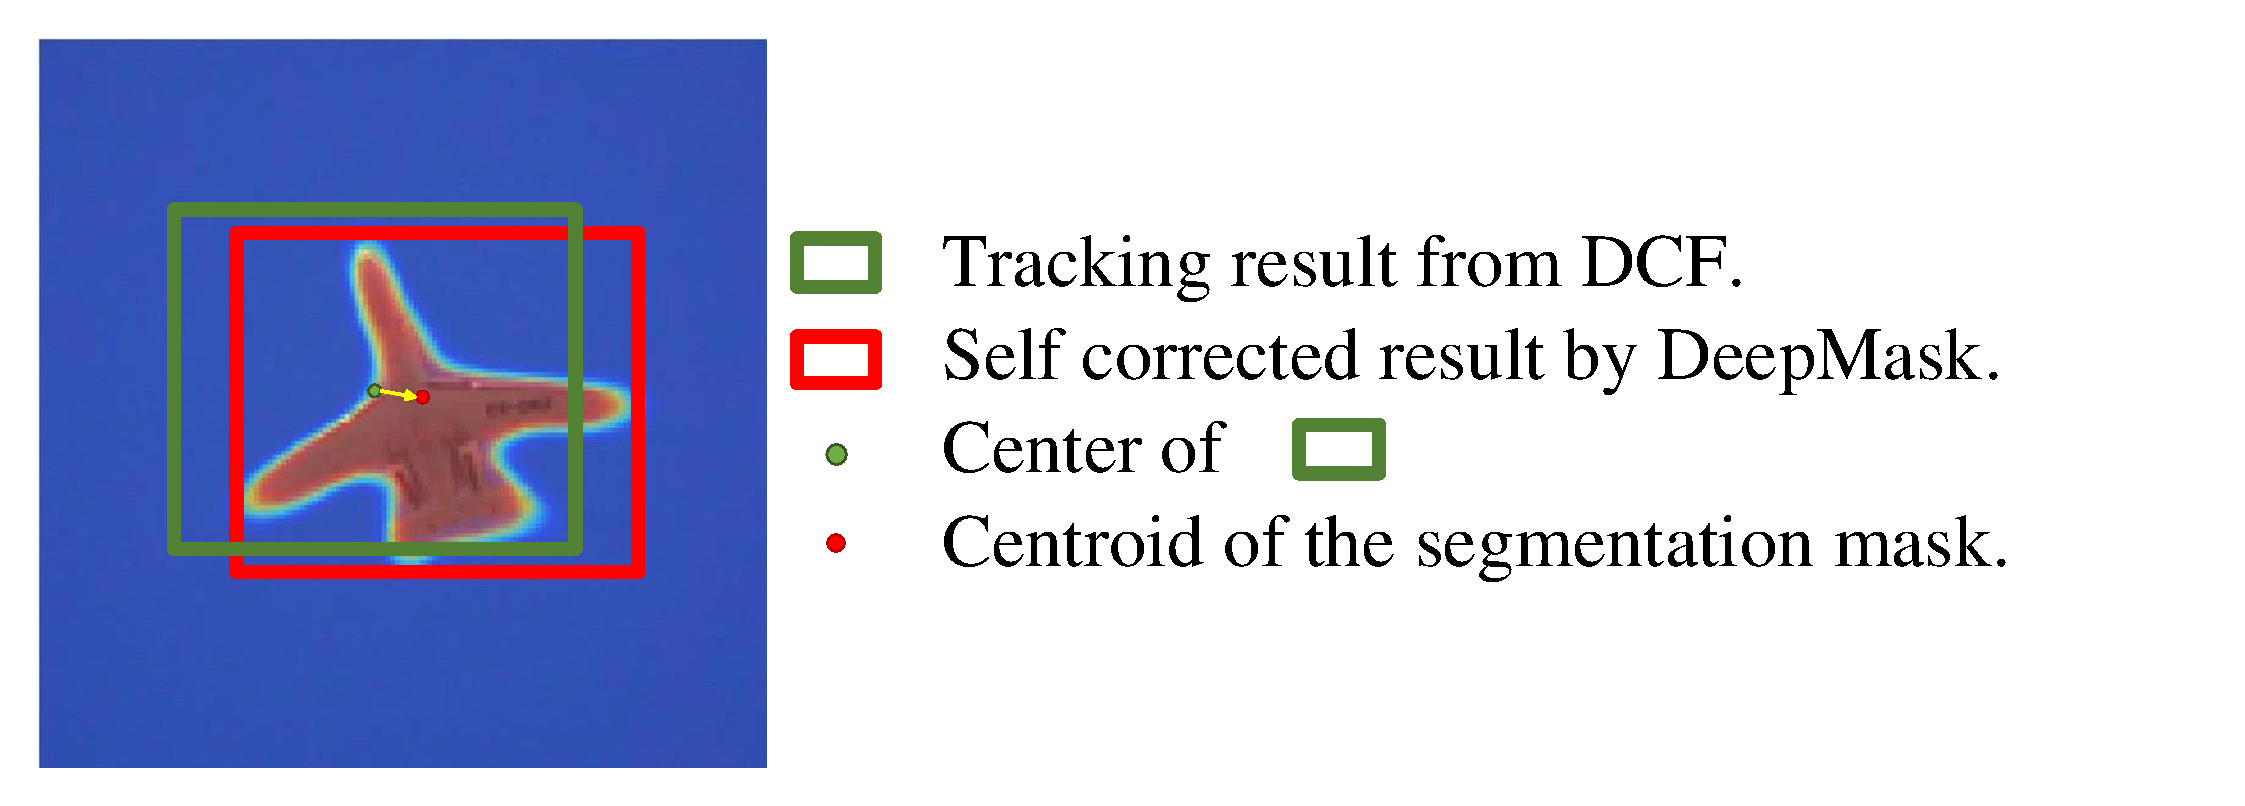
\includegraphics[width=1.0\textwidth]{Img/IGCF/cog_arch.pdf}
    \caption{实例引导的自纠正原理图。}
    \label{fig:net}
\end{figure*}

InstMask 允许学习更好的滤波器,并有助于纠正不良的跟踪结果。
在 DCF 模块中,滤波器 $h$ 和特征 $f$ 之间的最大相关位置被认为是当前帧中的目标位置。但是,由于在线更新,相关滤波器很容易漂移。
InstMask 的结果是根据从 COCO 数据集中获取的网络参数生成的。但是,由于 InstMask 不会在线更新,因此我们不能仅依靠目标的语义分割掩码来产生最终的跟踪结果。
为了利用两个结果的优点并克服它们的缺点,我们建议使用 \textbf{I}nstance \textbf{G}uided \textbf{S}elf-\textbf{C}orrection 组件 IGSC。IGSC 结合了这两个结果,以获得更好的跟踪。具体来说,使用硬阈值 $m$ 根据 $P$ 生成掩码 $b \in [0, 1] $:
\begin{equation}
m_{x,y} = \left\{ \begin{array}{ll}
 1 & \textrm{if $P_{x,y} > b$}\\
 0 & \textrm{if $P_{x,y} \le b$}
 \end{array} \right.
\end{equation}
$P$ 是从 InstMask 生成的概率图。元素 $P_{x,y}$ 是像素 $(x,y)$ 属于目标的概率。
然后从 $m$ 获得目标排名:
\begin{equation}
c_{m} = Centroid(m),
\end{equation}
其中 $Centroid(\mathord{\cdot})$ 可以计算区域的几何中心。
将 $p$ 表示为校正后的目标排名。
自校正过程可以描述如下:
\begin{equation}
p = \left\{ \begin{array}{ll}
 c_{m} & \textrm{if $||c_{m}-c_{dcf}||_2^2 < \beta$}\\
 c_{dcf} + \alpha \cdot (c_{m}-c_{dcf}) & \textrm{otherwise}
 \end{array} \right.,
\end{equation}
其中 $c_{dcf}$ 是 DCF 预测的位置,$\alpha$ 是控制自校正强度的超参数,而 $\beta$ 之间距离的阈值 $c_{m}$ 和 $c_{dcf}$。
由于分割结果的鲁棒性,当 DCF 结果显示不稳定漂移时,跟踪器可以自行校正。图 \ref{fig:IGSC} 中显示了提出的实例指导的自校正组件的有效性。

\iffalse
\begin{figure}[t]
\centering
    \subfloat{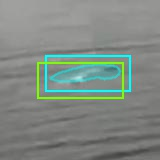
\includegraphics[width=2.45cm]{Img/IGCF/cog/birds1/00003.jpg}}          \hspace{-0.6em}        
    \subfloat{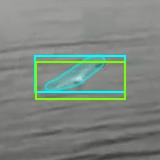
\includegraphics[width=2.45cm]{Img/IGCF/cog/birds1/00005.jpg}}          \hspace{-0.6em}        
    \subfloat{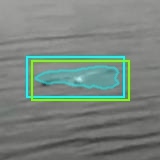
\includegraphics[width=2.45cm]{Img/IGCF/cog/birds1/00007.jpg}}          \hspace{-0.6em}        
    \subfloat{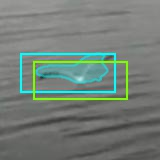
\includegraphics[width=2.45cm]{Img/IGCF/cog/birds1/00013.jpg}}          \hspace{-0.6em}        
    \subfloat{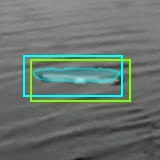
\includegraphics[width=2.45cm]{Img/IGCF/cog/birds1/00057.jpg}}\\[0.2ex]
    \subfloat{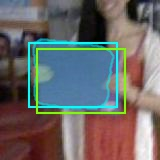
\includegraphics[width=2.45cm]{Img/IGCF/cog/book/00002.jpg}}                     \hspace{-0.6em}
    \subfloat{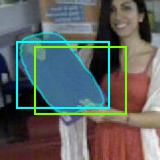
\includegraphics[width=2.45cm]{Img/IGCF/cog/book/00005.jpg}}                     \hspace{-0.6em}
    \subfloat{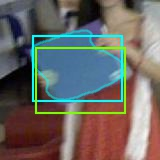
\includegraphics[width=2.45cm]{Img/IGCF/cog/book/00011.jpg}}                     \hspace{-0.6em}
    \subfloat{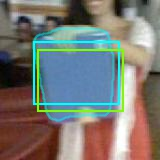
\includegraphics[width=2.45cm]{Img/IGCF/cog/book/00013.jpg}}                     \hspace{-0.6em}    \subfloat{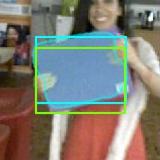
\includegraphics[width=2.45cm]{Img/IGCF/cog/book/00016.jpg}}\\[0.2ex]
    \subfloat{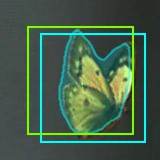
\includegraphics[width=2.45cm]{Img/IGCF/cog/butterfly/00015.jpg}}                   \hspace{-0.6em}
    \subfloat{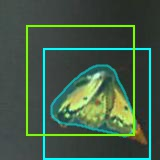
\includegraphics[width=2.45cm]{Img/IGCF/cog/butterfly/00019.jpg}}                   \hspace{-0.6em}
    \subfloat{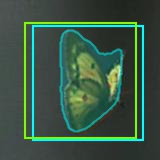
\includegraphics[width=2.45cm]{Img/IGCF/cog/butterfly/00025.jpg}}                   \hspace{-0.6em}
    \subfloat{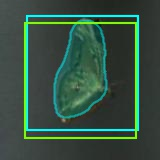
\includegraphics[width=2.45cm]{Img/IGCF/cog/butterfly/00027.jpg}}                   \hspace{-0.6em}
    \subfloat{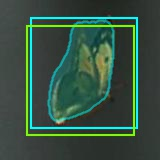
\includegraphics[width=2.45cm]{Img/IGCF/cog/butterfly/00031.jpg}}
    \caption{实例指导(自我校正)组件之前(绿色)和之后(蓝色)的跟踪结果。}
    \label{fig:IGSC}
\end{figure}
\fi

\begin{figure}
\centering
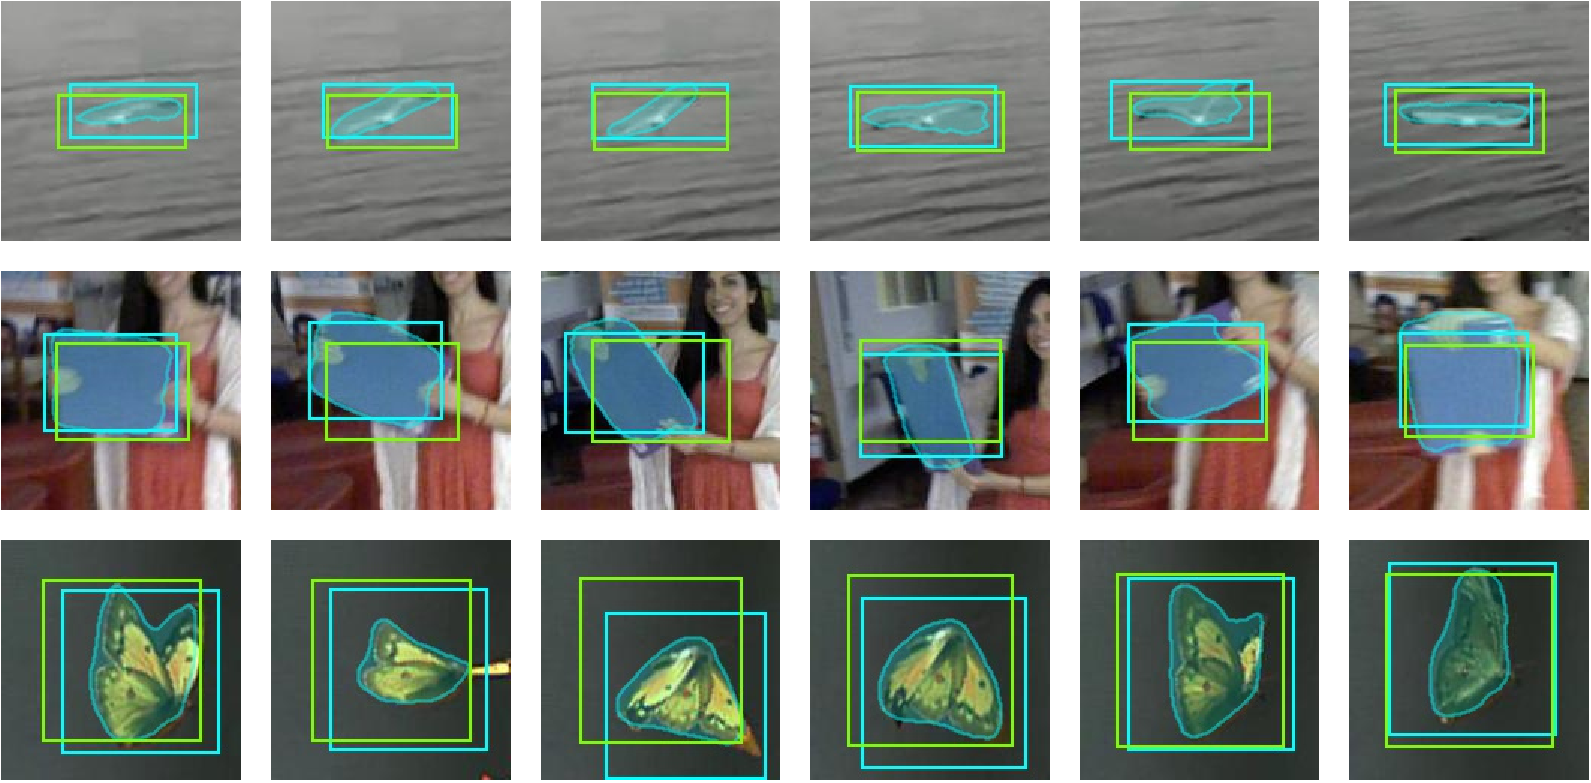
\includegraphics[width=1.0\textwidth]{Img/IGCF/cog.pdf}
\caption{实例指导(自我校正)组件之前(绿色)和之后(蓝色)的跟踪结果。}
\end{figure}

\subsection{总览}
跟踪过程包括两个阶段:本地化和模型更新。
在定位阶段,目标位置 $p_t$ 是相关的结果的最大位置:$h_{t-1}$ 和图像补丁特征 $f$ 从如下位置提取 $p_{t-1}$ 并根据通道依赖性得分加权 $w$ (等式 \ref{eq:dcf})。
分割掩码 $m$ 使用提出的 InstMask 网络估计 (第 \ref{sec:InstMask} 节)。
分割掩码的质心用于校正相关滤波器的预测偏差 (第 \ref{sec:cog} 节)。
然后新的尺度 $s_t$ 由单个比例空间相关滤波器估计(参见 \cite{Danelljan2014AccurateSE})。
信道检测可靠性 $\tilde{w}^{(det)}$ 估算如下 \cite{Lukezic2017DiscriminativeCF}:
\begin{equation} \label{eq:det}
\tilde w_d^{(det)} = max(1 - \rho_d^{max2} / \rho_d^{max1}, 0.5),
\end{equation}
这反映了每个渠道为一个目标位置投票的唯一性。$\tilde w_d^{(det)}$ 用于稍后计算 $w$ (等式 \ref{eq:c})。$\rho_d^{max2}$ 和 $\rho_d^{max1}$ 分别是通道 $d$的相关响应中第二高的非相邻峰值。

在模型更新阶段,新的滤波器 $\tilde{h}$ 使用模板 $m$ 进行估计。我们使用 \cite{Lukezic2017DiscriminativeCF} 中提出的迭代方法来有效地解决滤波器。令 $l$ 为拉格朗日乘数,$\mu > 0$,$h_m=m \odot h$,$\hat{h}^0 = h_{t-1}$ 和 $\hat{l}^0 = 0$。在每次迭代中,都按照 \cite{Lukezic2017DiscriminativeCF}中的顺序依次解决以下子问题:
\begin{equation} \label{eq:h1}
\hat{h}_c^{i+1} = \frac{\hat{f} \odot \bar{\hat{g}} +(\mu^i \hat{h}_m^i - \hat{l}^i)}{\bar{\hat{f}} \odot \hat f + \mu^i}
\end{equation}
\begin{equation}
h^{i+1} = \frac{m \odot \mathcal{F}^{-1}[\hat{l}^i + \mu^i\hat{h}_c^{i+1}]}{\frac{\lambda}{2D} + \mu^i}
\end{equation}
\begin{equation} \label{eq:h3}
\hat{l}^{i+1} = \hat{l}^i + \mu(\hat{h}_c^{i+1} - \hat{h}^{i+1})
\end{equation}
然后计算信道可靠性 $\tilde w_d$ \cite{Lukezic2017DiscriminativeCF} ,其中包括信道学习可靠性 $\tilde w_d^{(lrn)}$ 和信道检测可靠性 $\tilde w_d^{(det)}$ 如下: 
\begin{equation} \label{eq:c}
\tilde w_d = \tilde w_d^{(lrn)} \cdot \tilde w_d^{(det)},
\end{equation}
其中 $\tilde{w}^{(lrn)}$ 表示学习的信道滤波器的最大响应值:
\begin{equation} \label{eq:lrn}
\tilde{w}_d^{lrn} = max(f_d * h_d).
\end{equation}
最后,滤波器和通道可靠性在线更新:\begin{equation} \label{eq:update1}
h_t = (1 - \eta)h_{t-1} + \eta \tilde{h}
\end{equation}
\begin{equation} \label{eq:update2}
w_t = (1-\eta)w_{t-1} + \eta \tilde{w},
\end{equation}
其中 $\eta$ 是用于控制模型更新速度的学习率。

\begin{figure}[t]
    \centering
    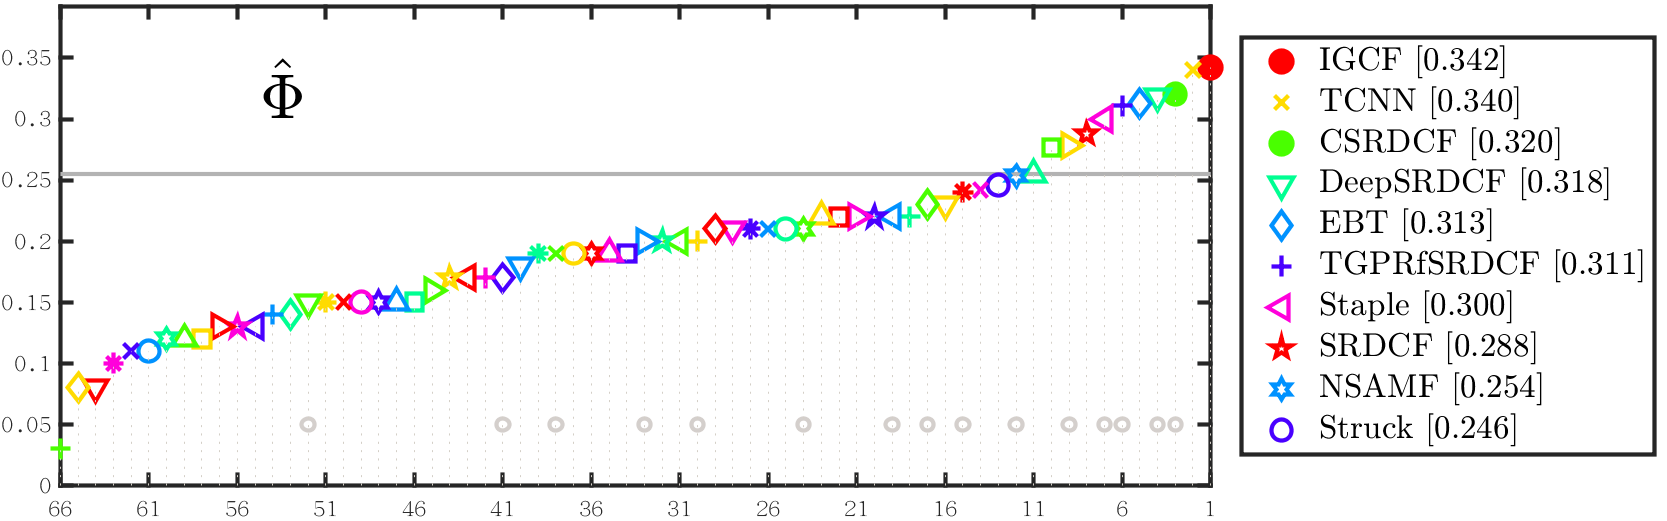
\includegraphics[width=1.0\textwidth]{Img/IGCF/vot/eao_rank_vot2015.png}
    \caption{VOT2015的预期平均重叠(EAO)图 \cite{Kristan2015TheVO}.}
    \label{fig:vot15}
\end{figure}

\begin{figure}[t]
    \centering
    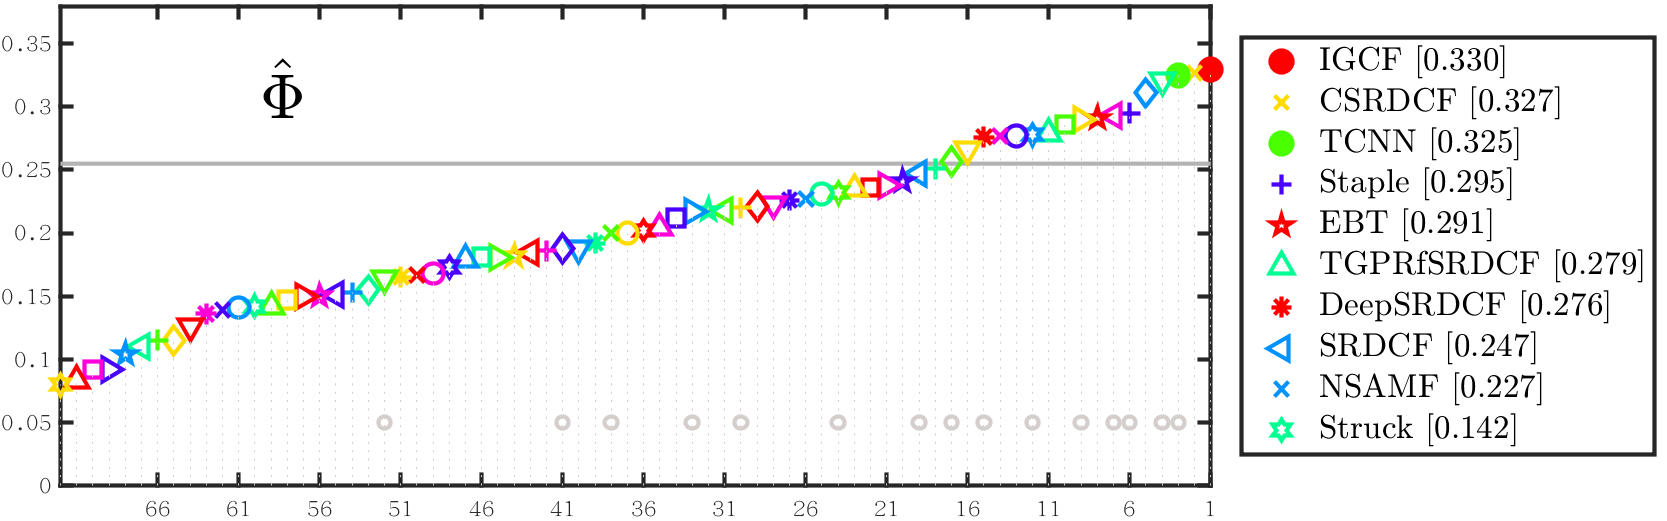
\includegraphics[width=1.0\textwidth]{Img/IGCF/vot/eao_rank_vot2016.png}
    \caption{VOT2016 的预期平均重叠(EAO)图 \cite{Kristan2016TheVO}。}
    \label{fig:vot16}
\end{figure}

\section{实验}
我们在三个具有挑战性的目标跟踪数据集上对拟议的跟踪器IGCF进行了全面评估:VOT2015 \cite{Kristan2015TheVO},VOT2016 \cite{Kristan2016TheVO} 和 GOT-10k \cite{GOT-10k}。请注意,用于训练 InstMask 组件的视频与评估数据集之间没有重叠。另外,对视频目标分割数据集DAVIS \cite{Perazzi2016}进行了定性实验。
\subsection{对 VOT2015 的评估}

\begin{figure}[t]
    \centering
    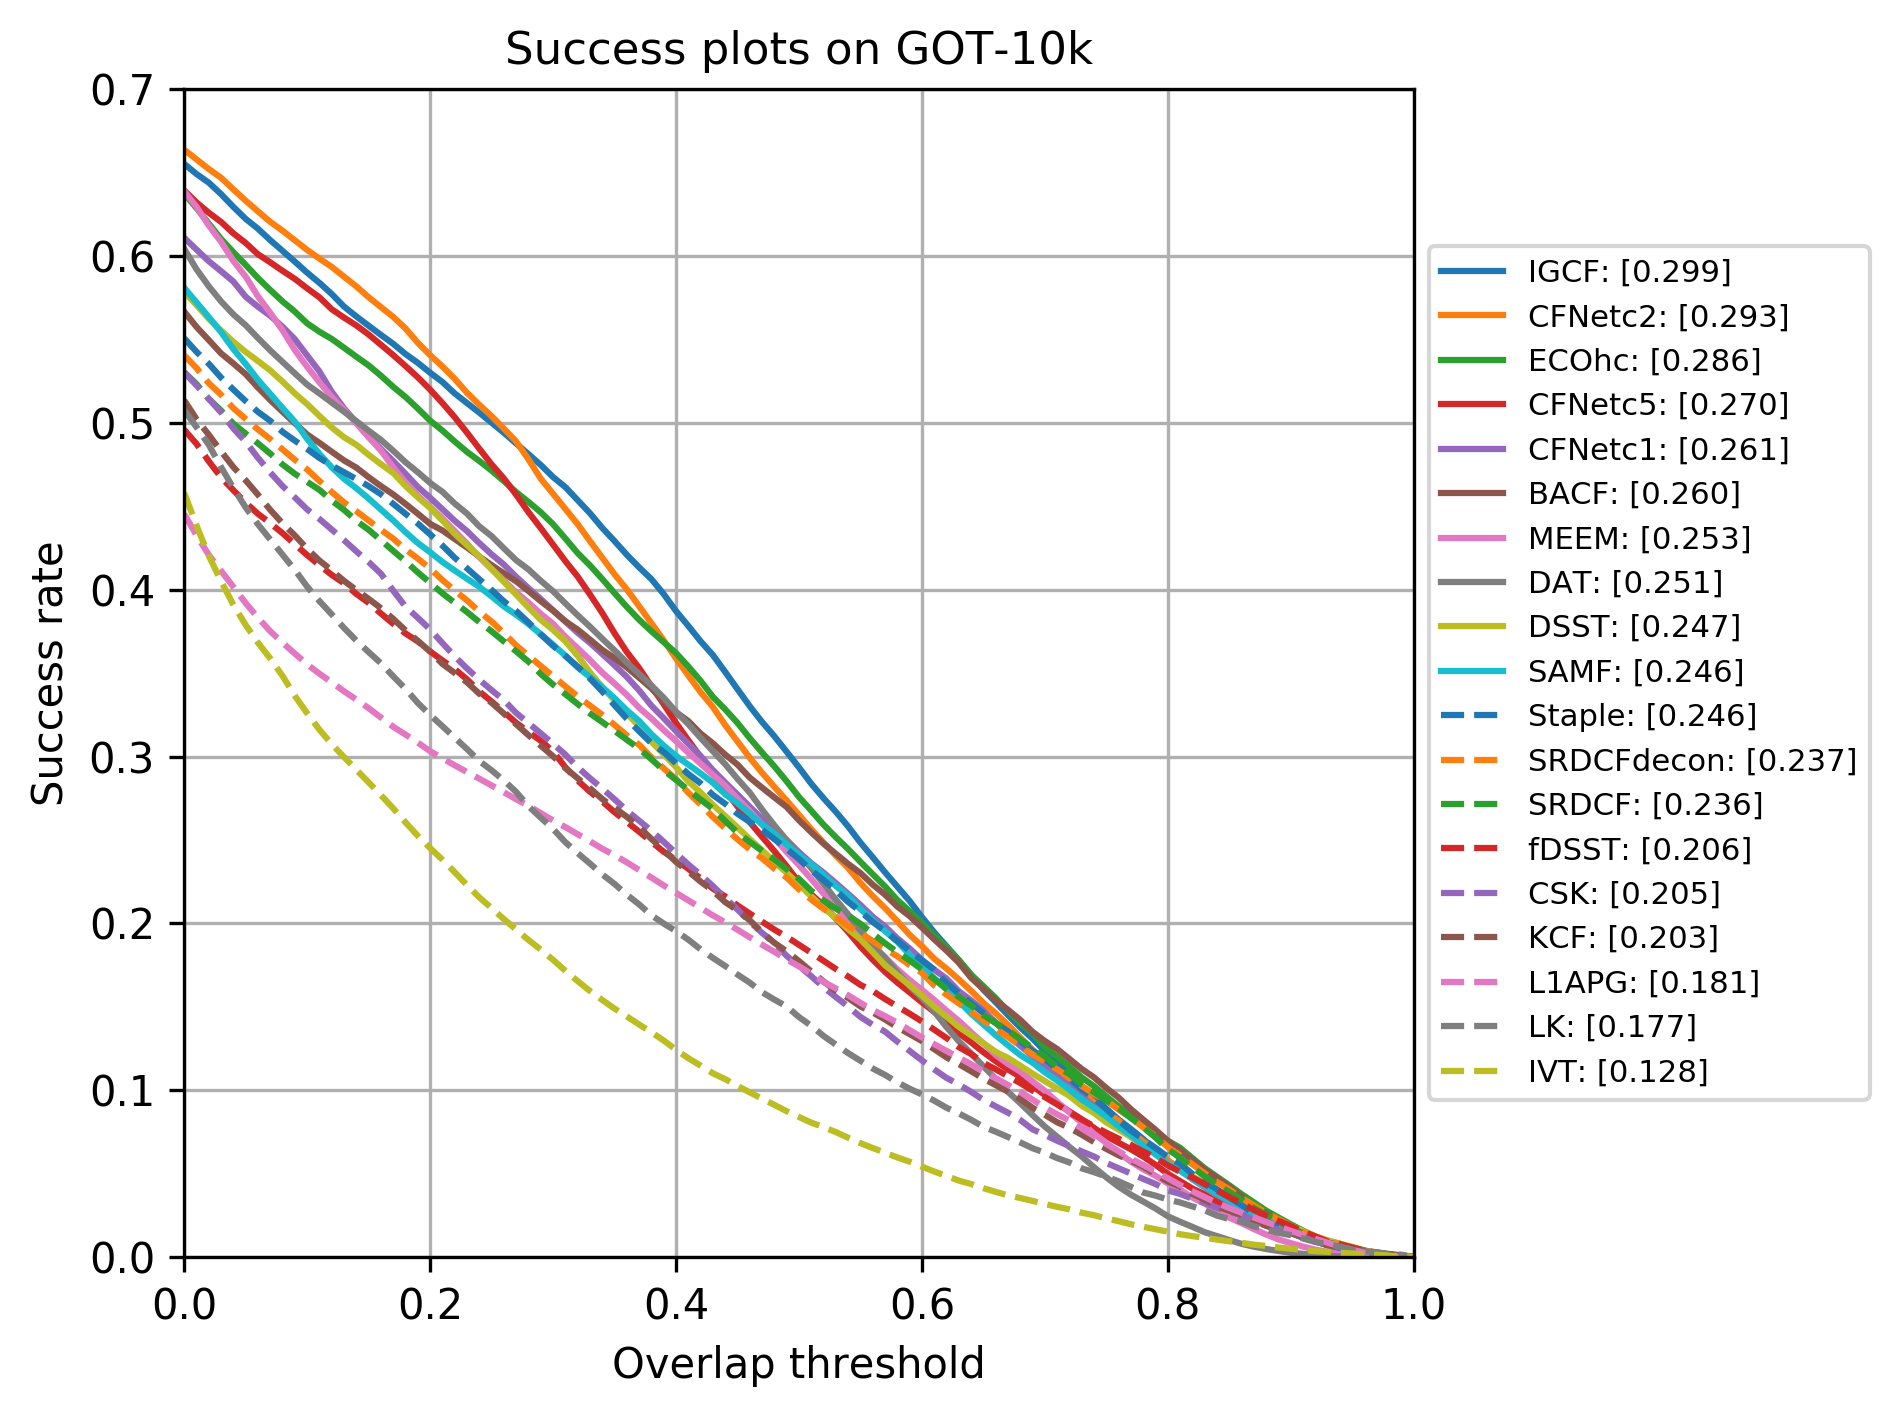
\includegraphics[width=0.8\textwidth]{Img/IGCF/got10k/success_plot.png}
    \caption{在 GOT-10k \cite{GOT-10k}上的总体性能,按其平均重叠(AO)得分进行排名。}
    \label{fig:got10k}
\end{figure}

VOT2015 \cite{Kristan2015TheVO} 跟踪数据集包含 60 个具有挑战性的视频。它是通过先进的序列选择方法从 300 多个序列中构建的,该方法优先处理难以追踪的目标并最大化视觉属性多样性成本函数。
在 VOT2015 中,使用三个指标来评估跟踪器的性能:(1)准确性,(2)鲁棒性和(3)EAO(预期平均重叠)。精度衡量跟踪器预测的边界框与地面真值边界框的重叠程度。健壮性衡量跟踪器在跟踪过程中失去目标(失败)的次数。EAO 结合了准确性和鲁棒性来评估跟踪器的整体性能。

我们将我们的算法与以下跟踪器进行了比较:CSRDCF \cite{Lukezic2017DiscriminativeCF},SRDCF \cite{Danelljan2015LearningSR},TGPRfSRDCF \cite{gao2018tracking},DeepSRDCF \cite{Danelljan2015ConvolutionalFF},TCNN \cite{nam2016modeling},Staple \cite{Bertinetto2016StapleC}, EBT \cite{Zhu2016BeyondLS},NSAMF \cite{Hua2015OnlineOT} 和 Struck \cite{Hare2011StruckSO}.
这些跟踪器可以分为三类:Struck 和 EBT 是传统的跟踪器。SRDCF,CSRDCF,TGPRfSRDCF,Staple 和 SAMF 是基于 DCF 的跟踪器。DeepSRDCF 和 TCNN 是基于 CNN 的跟踪器。
跟踪器的 EAO 得分如图 \ref{fig:vot15}。与其他列出的方法相比,我们的方法可实现 0.342 的出色 EAO。
Struck 使用内核化的结构化输出支持向量机(SVM),可以在线学习以提供自适应跟踪。相反,IGCF 基于强大的相关滤波器。因此,IGCF 在EAO 方面的相对提升显著优于 Struck,达到 36.8%,这表明 DCF 框架的出色表现以及 IGCF 的有效性。
CSRDCF 使用目标和背景的颜色直方图生成目标掩码,以限制相关滤波器的学习,而 IGCF 使用神经网络生成掩码。与 CSRDCF 相比,EAO 分数的相对提高为 6.9%,这表明,与使用底层图像特征生成的掩码相比,使用深层卷积特征生成的语义掩码更有利于滤波器的学习。
DeepSRDCF 在 SRDCF 框架中结合了来自预训练网络的深层卷积特征。但是,所使用的深层特征并不专用于实例分割。相比之下,InstMask 在针对实例分割而设计的 COCO 分割数据集上进行了训练。在 VOT2015 上,就 EAO 而言,IGCF 比 DeepSRCDF 高出 7.5%,这强调了提出的的 InstMask 和 IGSC 模块的重要性。

\subsection{对 VOT2016 的评估}
VOT2016 \cite{Kristan2016TheVO} 数据集包含来自 VOT2015 的 60 个序列,具有改进的注释。VOT2016 的评估指标与 VOT2015 相同,即准确性,鲁棒性和 EAO。

我们将所提出的算法与以下跟踪器进行了比较:
CSRDCF \cite{Lukezic2017DiscriminativeCF},SRDCF \cite{Danelljan2015LearningSR},TGPRfSRDCF \cite{gao2018tracking},DeepSRDCF \cite{Danelljan2015ConvolutionalFF},TCNN \cite{nam2016modeling}, Staple \cite{Bertinetto2016StapleC},EBT \cite{Zhu2016BeyondLS},NSAMF \cite{Hua2015OnlineOT} 和 Struck \cite{Hare2011StruckSO}。图 \ref{fig:vot16} 显示了 VOT2016 上 EAO 的性能。在比较的方法中,我们的方法以 0.330 的 EAO 得分达到最佳结果。

\subsection{对 GOT-10k 的评估}
GOT-10k \cite{GOT-10k} 是近期提出的用于通用目标跟踪的数据库。该数据集包含超过 10000 个真实运动目标的视频片段和超过 150 万个手动标记的边界框。现实世界中有 563 类运动目标和 87 种运动模式。
我们在 GOT-10k 测试子集上评估跟踪器,包括 180 段视频,具有 84 个目标类别和 32 个运动模式。
GOT-10k 的评估指标是平均重叠(AO),它表示所有地面和估计边界框之间重叠的平均值。

我们将本文提出的 IGCF 算法与以下跟踪器进行了比较:CFNetc2 \cite{Valmadre2017EndtoEndRL},ECOhc \cite{Danelljan2017ECOEC},CFNetc5 \cite{Valmadre2017EndtoEndRL},CFNetc1 \cite{Valmadre2017EndtoEndRL}, BACF \cite{Galoogahi2017LearningBC},MEEM \cite{Zhang2014MEEMRT},DAT \cite{Possegger2015InDO},DSST \cite{Danelljan2014AccurateSE},SAMF \cite{Li2014ASA},Staple \cite{Bertinetto2016StapleC},SRDCFdecon \cite{Danelljan2016AdaptiveDO},SRDCF \cite{Danelljan2015LearningSR},fDSST \cite{Danelljan2017DiscriminativeSS},CSK \cite{Henriques2012ExploitingTC},KCF \cite{henriques2014high-speed},L1APG \cite{Bao2012RealTR},LK \cite{Shi1994GoodFT} 和 IVT \cite{Ross2007IncrementalLF}。评估的跟踪器的成功图如图 \ref{fig:got10k}所示。它代表重叠度量超过阈值的帧相对于不同阈值的百分比。我们的方法的 AO 得分为 0.299,优于所有其他列出的竞争跟踪算法。

\begin{figure}[t]
\centering
    \subfloat{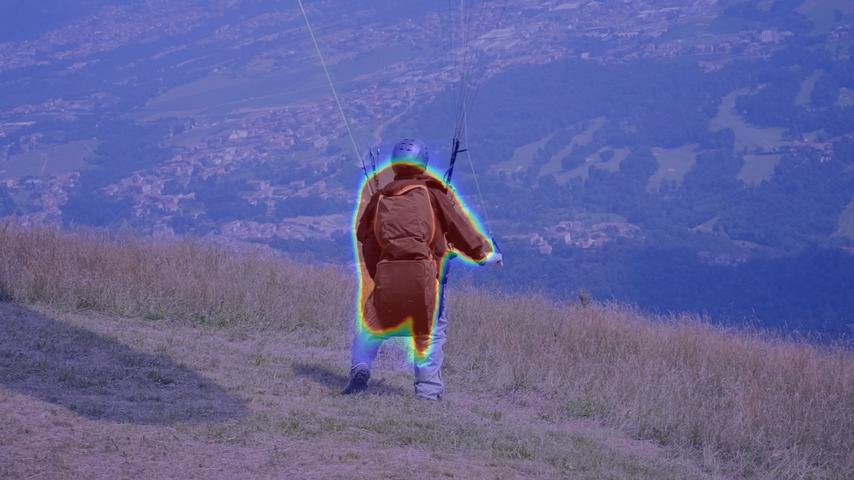
\includegraphics[width=2.43cm]{Img/IGCF/davis16val/paragliding-launch/00001.jpg}}          \hspace{-0.6em}        
    \subfloat{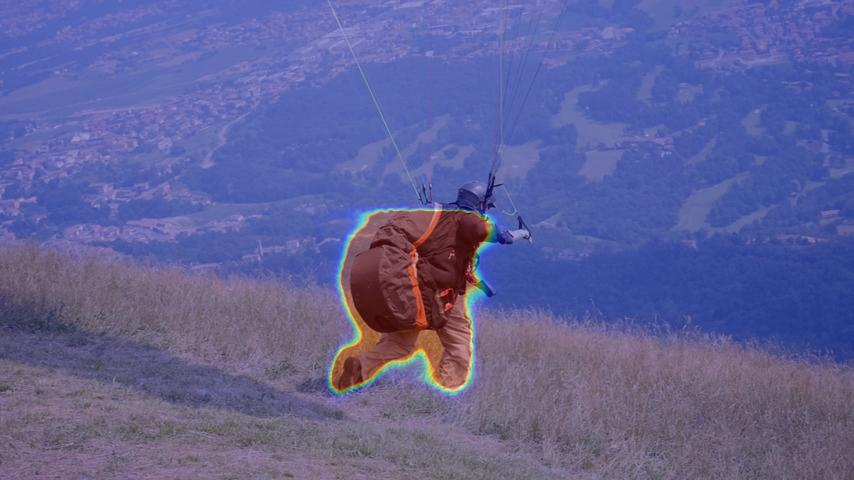
\includegraphics[width=2.43cm]{Img/IGCF/davis16val/paragliding-launch/00021.jpg}}          \hspace{-0.6em}        
    \subfloat{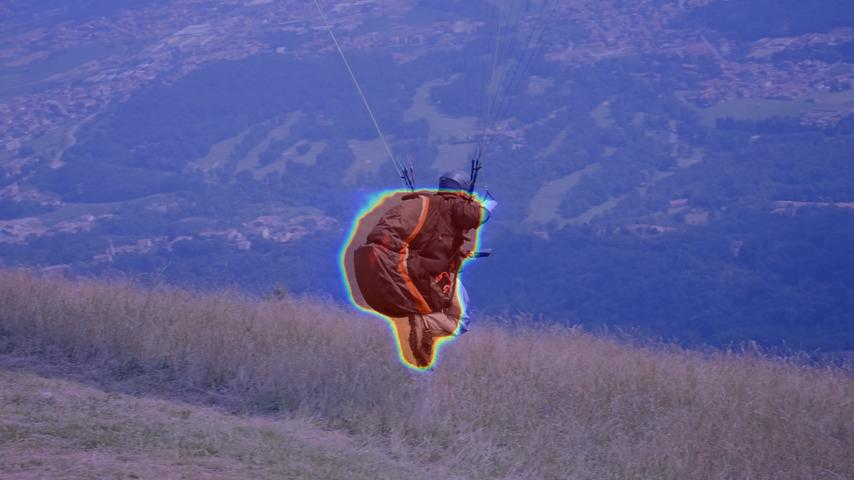
\includegraphics[width=2.43cm]{Img/IGCF/davis16val/paragliding-launch/00032.jpg}}          \hspace{-0.6em}        
    \subfloat{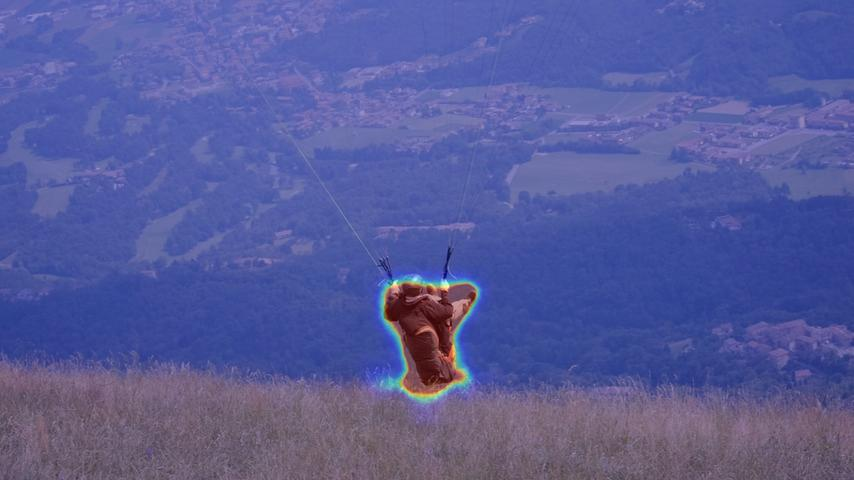
\includegraphics[width=2.43cm]{Img/IGCF/davis16val/paragliding-launch/00069.jpg}}          \hspace{-0.6em}        
    \subfloat{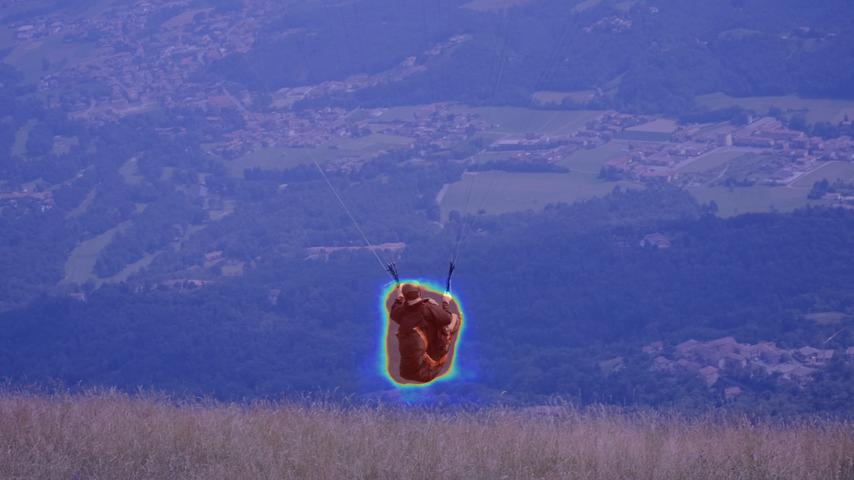
\includegraphics[width=2.43cm]{Img/IGCF/davis16val/paragliding-launch/00079.jpg}}\\[0.2ex]
    \subfloat{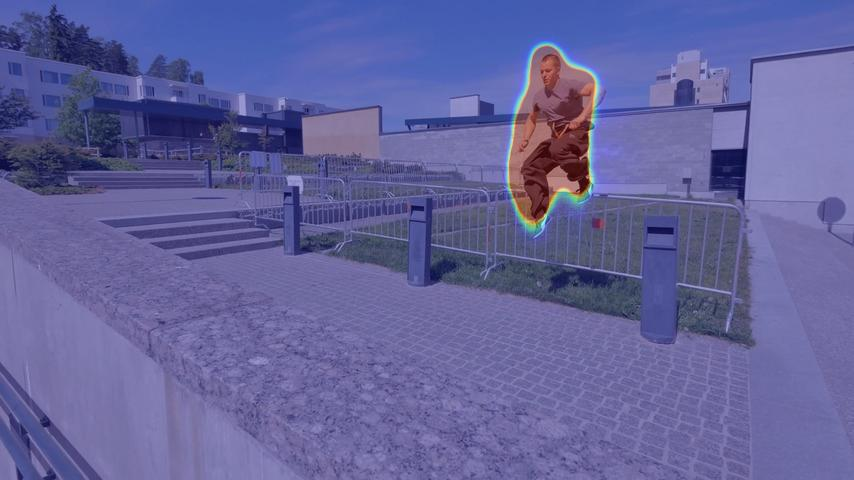
\includegraphics[width=2.43cm]{Img/IGCF/davis16val/parkour/00001.jpg}}                     \hspace{-0.6em}
    \subfloat{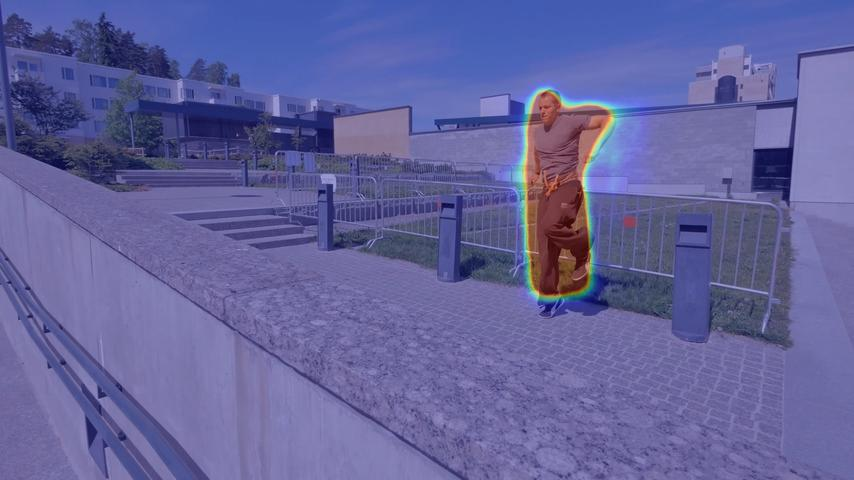
\includegraphics[width=2.43cm]{Img/IGCF/davis16val/parkour/00006.jpg}}                     \hspace{-0.6em}
    \subfloat{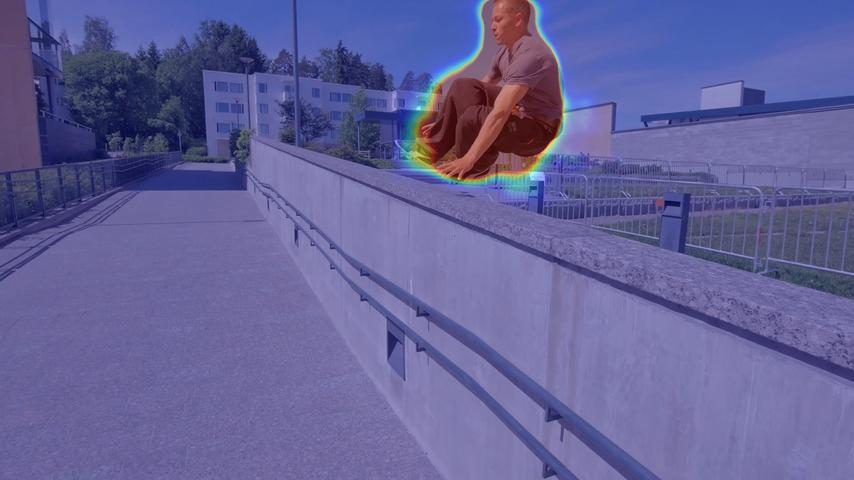
\includegraphics[width=2.43cm]{Img/IGCF/davis16val/parkour/00026.jpg}}                     \hspace{-0.6em}
    \subfloat{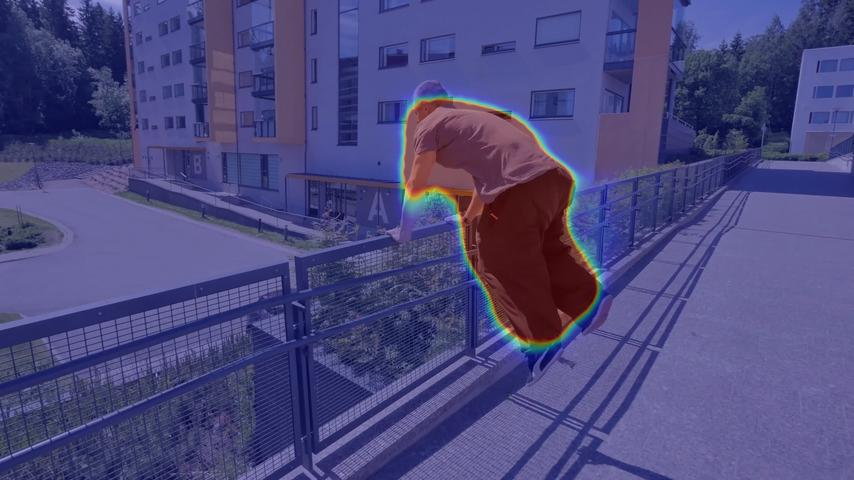
\includegraphics[width=2.43cm]{Img/IGCF/davis16val/parkour/00063.jpg}}                     \hspace{-0.6em}
    \subfloat{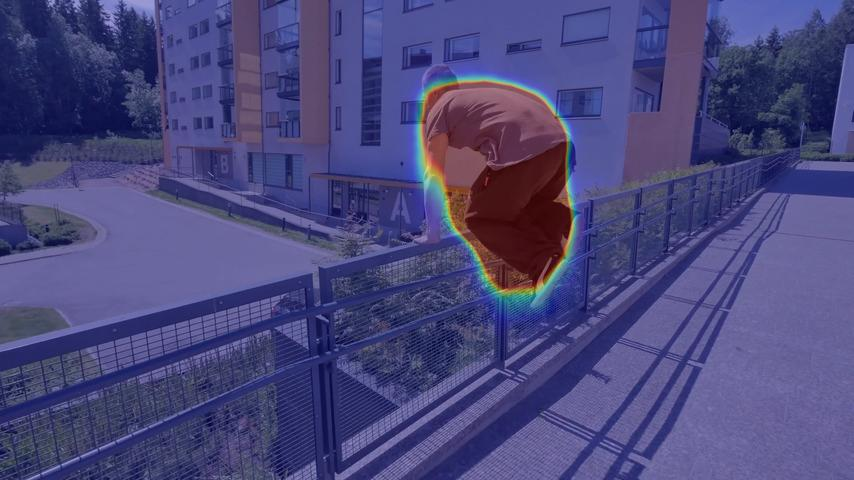
\includegraphics[width=2.43cm]{Img/IGCF/davis16val/parkour/00065.jpg}}\\[0.2ex]
    \subfloat{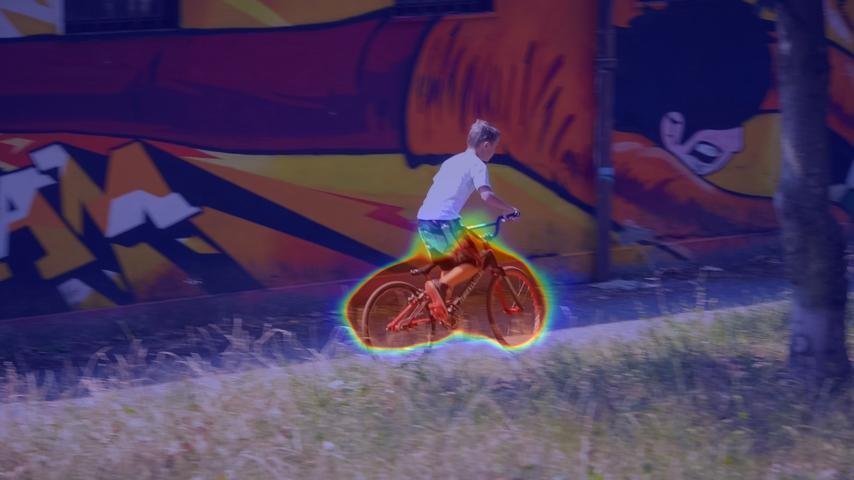
\includegraphics[width=2.43cm]{Img/IGCF/davis16val/bmx-trees/00001.jpg}}                   \hspace{-0.6em}
    \subfloat{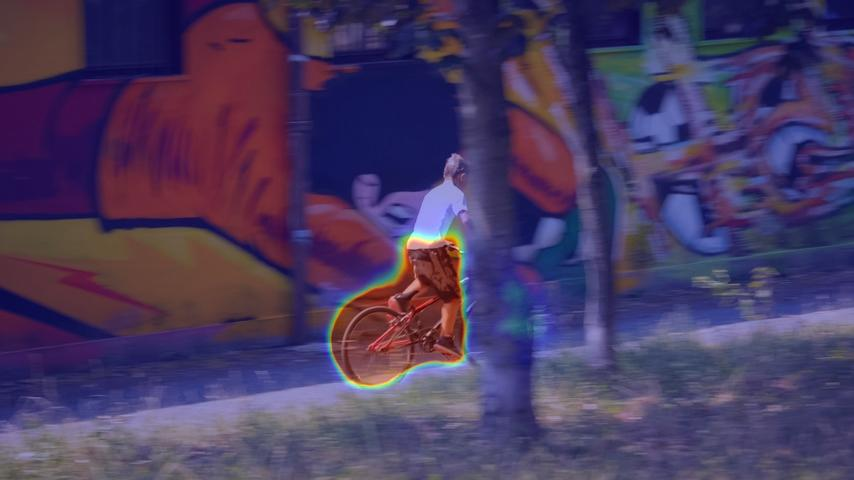
\includegraphics[width=2.43cm]{Img/IGCF/davis16val/bmx-trees/00014.jpg}}                   \hspace{-0.6em}
    \subfloat{\includegraphics[width=2.43cm]{Img/IGCF/davis16val/bmx-trees/00017.jpg}}                   \hspace{-0.6em}
    \subfloat{\includegraphics[width=2.43cm]{Img/IGCF/davis16val/bmx-trees/00036.jpg}}                   \hspace{-0.6em}
    \subfloat{\includegraphics[width=2.43cm]{Img/IGCF/davis16val/bmx-trees/00067.jpg}}
    \caption{我们的方法在 DAVIS2016 VAL 数据集中的定性结果。}
    \label{fig:davis}
\end{figure}


\subsection{对 DAVIS2016 的评估}
配备有 InstMask 模块的跟踪器不仅可以很好地执行目标跟踪,还可以用于视频分割。DAVIS \cite{Perazzi2016} 是一个视频目标分割数据集,它由 50 个高质量视频序列组成,跨越了多次出现的常见视频目标分割挑战,例如遮挡,运动模糊和外观变化。我们在 DAVIS2016 的验证集上进行了定性实验。可视化结果如图 \ref{fig:davis}所示。结果表明,提出的 IGCF 可以准确地恢复目标的轮廓,这在一定程度上解释了 IGCF 为什么可以提高跟踪性能。

\section{结论}
在本文中,我们提出了一种新颖的跟踪器,该跟踪器结合了深度神经网络和相关滤波器的优点来提高目标跟踪的性能。
InstMask 用于约束相关滤波器的学习过程。基于实例级别的分割,我们进一步提出了一种自校正机制,以减轻对相关滤波器的漂移。
通过与最新的跟踪器进行比较,实验结果显示了该方法的出色鲁棒性和效率。